\documentclass[12pt]{article}

\usepackage[top=1in, bottom=1in, left=1in, right=1in]{geometry} 
\usepackage{graphicx}
\usepackage{setspace}
\usepackage{bm}
\usepackage{amsmath}
\usepackage{amssymb,amsmath}
\usepackage{listings}
\usepackage{titling}
\usepackage{color}
\usepackage{enumitem}
\usepackage{fancyvrb}
\usepackage{hyperref}
\usepackage{diagbox}
\usepackage{float}
\geometry{letterpaper}
\linespread{1.1}% \geometry{landscape} % rotated page geometry

\definecolor{codegreen}{rgb}{0,0.6,0}
\definecolor{codegray}{rgb}{0.5,0.5,0.5}
\definecolor{codepurple}{rgb}{0.58,0,0.82}
\definecolor{backcolour}{rgb}{0.95,0.95,0.92}
\definecolor{outcolor}{rgb}{0.545, 0.0, 0.0}

\lstdefinestyle{mystyle}{
	backgroundcolor=\color{backcolour},   
	commentstyle=\color{codegreen},
	keywordstyle=\color{magenta},
	numberstyle=\tiny\color{codegray},
	stringstyle=\color{codepurple},
	basicstyle=\footnotesize,
	breakatwhitespace=false,         
	breaklines=true,                 
	captionpos=b,                    
	keepspaces=true,                 
	numbers=left,                    
	numbersep=5pt,                  
	showspaces=false,                
	showstringspaces=false,
	showtabs=false,                  
	tabsize=2
}

\lstset{style=mystyle}
\setlength{\droptitle}{1cm}
\title{HW 3: Optimal Economic Dispatch in Distribution Feeders with Renewables}
\date{14 Mar. 2018} 
\author{Franklin Zhao \\ SID: 3033030808}

\begin{document}
	
	\maketitle
	\newcommand{\tabitem}{~~\llap{\textbullet}~~}
	\renewcommand\theequation{\arabic{equation}}
	\renewcommand{\figurename}{Fig.}
	\renewcommand\thesection{Problem \arabic{section}:}
	\renewcommand\thesubsection{(\alph{subsection})}
	\onehalfspacing
	
\section{Network Parameters}
\subsection{}
The plot of active and reactive power consumption is shown in Figure~\ref{fig:1}.
\begin{figure}[H]
\centering
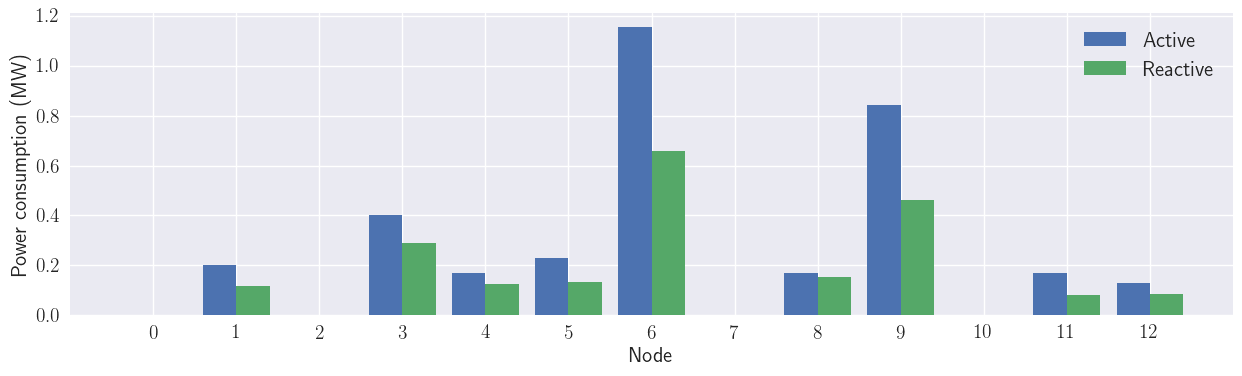
\includegraphics[width=\linewidth]{1.png}
\vspace{-1cm}      
\caption{Active and reactive power consumption}
\label{fig:1}
\end{figure}
\newpage
\subsection{}
The adjacency matrix is shown as follow:
\begin{verbatim}				
0	1	0	0	0	0	0	0	0	0	0	0	0
0	0	1	0	1	0	1	0	0	0	0	0	0
0	0	0	1	0	0	0	0	0	0	0	0	0
0	0	0	0	0	0	0	0	0	0	0	0	0
0	0	0	0	0	1	0	0	0	0	0	0	0
0	0	0	0	0	0	0	0	0	0	0	0	0
0	0	0	0	0	0	0	1	1	0	1	0	0
0	0	0	0	0	0	0	0	0	0	0	0	0
0	0	0	0	0	0	0	0	0	1	0	0	0
0	0	0	0	0	0	0	0	0	0	0	0	0
0	0	0	0	0	0	0	0	0	0	0	1	1
0	0	0	0	0	0	0	0	0	0	0	0	0
0	0	0	0	0	0	0	0	0	0	0	0	0
\end{verbatim}
\section{Balancing Supply \& Demand without a Network}
\subsection{}
Optimization variables:\\
$\bf{p}\in\mathbb{R}^{13}$ (where $p_i$ is the active power generated at node $i$)\\
$\bf{q}\in\mathbb{R}^{13}$ (where $q_i$ is the reactive power generated at node $i$)\\
$\bf{s}\in\mathbb{R}^{13}$ (where $s_i$ is the apparent power generated at node $i$)
\subsection{}
Objective function:\\
\begin{equation}
\sum_{i=0}^{12}c_is_i
\end{equation}
\newpage
\subsection{}
Constraint 1 (apparent power limits): 
\begin{equation}
s_i\leq s_{i,max}\ \ \ \ \ \forall i\in [0, 12]
\end{equation}
Constraint 2 (balance active power generation with consumption):
\begin{equation}
\sum_{i=0}^{12}p_i=\sum_{i=0}^{12}l_i^P
\end{equation}
Constraint 3 (balance reactive power generation with consumption):
\begin{equation}
\sum_{i=0}^{12}q_i=\sum_{i=0}^{12}l_i^Q
\end{equation}
Constraint 4 (power generation should be non-negative):
\begin{equation}
p_i\geq 0,\ \ q_i\geq 0 \ \ \ \ \ \forall i\in [0, 12]
\end{equation}
Constraint 5 (compute apparent power from active and reactive power):
\begin{equation}
\sqrt{p_i^2+q_i^2}=s_i \ \ \ \ \ \forall i\in [0, 12]
\end{equation}
\subsection{}
This problem is \textbf{not} a linear program (LP), \textbf{not} a quadratic program (QP), \textbf{not} a convex program (CP), since the Constrain 5 (a equality constraint) is not affine.\\\\
However, if we relax it to an inequality constraint, the problem will become a \textbf{CP} problem, since this inequality constraint is convex.
\newpage
\subsection{}
The result is shown as follow:
\begin{verbatim}
Minimum Generating Cost : 255.36 USD

Node 0 [Grid]  Gen Power : p_0 = 0.901 MW | q_0 = 0.546 MW | s_0 = 1.054 MW
Node 3 [Gas]   Gen Power : p_3 = 0.000 MW | q_3 = 0.000 MW | s_3 = 0.000 MW
Node 9 [Solar] Gen Power : p_9 = 2.565 MW | q_9 = 1.556 MW | s_9 = 3.000 MW

Total active power   : 3.466 MW   consumed | 3.466 MW   generated
Total reactive power : 2.102 MVAr consumed | 2.102 MVAr generated
Total apparent power : 4.063 MVA  consumed | 4.054 MVA  generated
\end{verbatim}
\section{Add Line Power Flows}
\subsection{}
Optimization variables:\\
$\bf{p}\in\mathbb{R}^{13}$ (where $p_i$ is the active power generated at node $i$)\\
$\bf{q}\in\mathbb{R}^{13}$ (where $q_i$ is the reactive power generated at node $i$)\\
$\bf{s}\in\mathbb{R}^{13}$ (where $s_i$ is the apparent power generated at node $i$)\\
$\bf{P}\in\mathbb{R}^{13\times13}$ (where $P_{ij}$ is the active power flowing on line ($i,j$)\\
$\bf{Q}\in\mathbb{R}^{13\times13}$ (where $Q_{ij}$ is the reactive power flowing on line ($i,j$)\\
\subsection{}
Constraint 1 (apparent power limits): 
\begin{equation}
s_i\leq s_{i,max}\ \ \ \ \ \forall i\in [0, 12]
\end{equation}
Constraint 2 (balance active power generation with consumption):
\begin{equation}
\sum_{i=0}^{12}p_i=\sum_{i=0}^{12}l_i^P
\end{equation}
Constraint 3 (balance reactive power generation with consumption):
\begin{equation}
\sum_{i=0}^{12}q_i=\sum_{i=0}^{12}l_i^Q
\end{equation}
Constraint 4 (power generation should be non-negative):
\begin{equation}
p_i\geq 0,\ \ q_i\geq 0 \ \ \ \ \ \forall i\in [0, 12]
\end{equation}
Constraint 5 (compute apparent power from active and reactive power (relaxed version)):
\begin{equation}
\sqrt{p_i^2+q_i^2}\leq s_i \ \ \ \ \ \forall i\in [0, 12]
\end{equation}
Constraint 6 (power flow should align with power generation and consumption at each node):
\begin{align}
P_{ij}=(l_j^P-p_j)+\sum_{k=0}^{12}A_{jk}P_{jk} \ \ \ \ \ \forall j\in [0, 12],\ i=\rho(j)\\
Q_{ij}=(l_j^Q-q_j)+\sum_{k=0}^{12}A_{jk}Q_{jk} \ \ \ \ \ \forall j\in [0, 12],\ i=\rho(j)
\end{align}
\subsection{}
The result is shown as follow:
\begin{verbatim}
Minimum Generating Cost : 255.36 USD

Node 0 [Grid]  Gen Power : p_0 = 0.901 MW | q_0 = 0.546 MW | s_0 = 1.054 MW || 
mu_s0 =   0 USD/MW
Node 3 [Gas]   Gen Power : p_3 = 0.000 MW | q_3 = 0.000 MW | s_3 = 0.000 MW || 
mu_s4 =   0 USD/MW
Node 9 [Solar] Gen Power : p_9 = 2.565 MW | q_9 = 1.556 MW | s_9 = 3.000 MW || 
mu_s9 =  50 USD/MW

Total active power   : 3.466 MW   consumed | 3.466 MW   generated
Total reactive power : 2.102 MVAr consumed | 2.102 MVAr generated
Total apparent power : 4.063 MVA  consumed | 4.054 MVA  generated
\end{verbatim}
\newpage
\noindent From the result we can notice that the minimum and minimizers remain the \textbf{same} as Problem 2. The reason is that when adding constraint 6, as we tune $P_{ij}$ and $Q_{ij}$, such a constraint will always be true no matter what $p_j$ or $q_j$ is, which means such a constraint have no connection to other constraints or the objective function. Hence, we actually did not ``add" a constraint compared to Problem 2 (This is an inactive constraint).
\subsection{} 
Actually in CVXPY we do not need to re-compute the problem
The result is shown as follow:
\begin{verbatim}
Minimum Generating Cost : 255.36 USD

Node 0 [Grid]  Gen Power : p_0 = 0.901 MW | q_0 = 0.546 MW | s_0 = 1.054 MW || 
mu_s0 =   0 USD/MW
Node 3 [Gas]   Gen Power : p_3 = 0.000 MW | q_3 = 0.000 MW | s_3 = 0.000 MW || 
mu_s4 =   0 USD/MW
Node 9 [Solar] Gen Power : p_9 = 2.565 MW | q_9 = 1.556 MW | s_9 = 3.000 MW || 
mu_s9 =  50 USD/MW

Total active power   : 3.466 MW   consumed | 3.466 MW   generated
Total reactive power : 2.102 MVAr consumed | 2.102 MVAr generated
Total apparent power : 4.063 MVA  consumed | 4.054 MVA  generated

Dual variable mu_s:
[[  1.19192177e-09]
[  1.36704047e+02]
[  1.37527656e+02]
[  1.26366831e-09]
[  1.37994308e+02]
[  1.38501208e+02]
[  1.40611644e+02]
[  1.40743436e+02]
[  1.40787583e+02]
[  5.32612423e-09]
[  1.41842060e+02]
[  1.42320563e+02]
[  1.42401951e+02]]
\end{verbatim}
If we increase the solar power capacity by 1MW, the reult is shown as follow:
\begin{verbatim}
Minimum Generating Cost : 205.36 USD

Node 0 [Grid]  Gen Power : p_0 = 0.046 MW | q_0 = 0.028 MW | s_0 = 0.054 MW || 
mu_s0 =   0 USD/MW
Node 3 [Gas]   Gen Power : p_3 = 0.000 MW | q_3 = 0.000 MW | s_3 = 0.000 MW || 
mu_s4 =   0 USD/MW
Node 9 [Solar] Gen Power : p_9 = 3.420 MW | q_9 = 2.074 MW | s_9 = 4.000 MW || 
mu_s9 =  50 USD/MW

Total active power   : 3.466 MW   consumed | 3.466 MW   generated
Total reactive power : 2.102 MVAr consumed | 2.102 MVAr generated
Total apparent power : 4.063 MVA  consumed | 4.054 MVA  generated
\end{verbatim}
As we can see from the reults above, we would save \textbf{50 USD} (nearly 20 percent!) if we could increase the solar power capacity by 1MW.
\section{The Complete Optimal Economic Dispatch with Distflow Equations}
\subsection{}
Optimization variables:\\
$\bf{p}\in\mathbb{R}^{13}$ (where $p_i$ is the active power generated at node $i$)\\
$\bf{q}\in\mathbb{R}^{13}$ (where $q_i$ is the reactive power generated at node $i$)\\
$\bf{s}\in\mathbb{R}^{13}$ (where $s_i$ is the apparent power generated at node $i$)\\
$\bf{P}\in\mathbb{R}^{13\times13}$ (where $P_{ij}$ is the active power flowing on line ($i,j$)\\
$\bf{Q}\in\mathbb{R}^{13\times13}$ (where $Q_{ij}$ is the reactive power flowing on line ($i,j$)\\
$\bf{V}\in\mathbb{R}^{13}$ (where $V_i$ is the squared magnitude of voltage at node $i$)\\
$\bf{L}\in\mathbb{R}^{13\times13}$ (where $L_{ij}$ is the squared magnitude of complex current on line ($i,j$))
\newpage
\subsection{}
Constraint 1 (apparent power limits): 
\begin{equation}
s_i\leq s_{i,max}\ \ \ \ \ \forall i\in [0, 12]
\end{equation}
Constraint 2 (balance active power generation with consumption):
\begin{equation}
\sum_{i=0}^{12}p_i=\sum_{i=0}^{12}l_i^P
\end{equation}
Constraint 3 (balance reactive power generation with consumption):
\begin{equation}
\sum_{i=0}^{12}q_i=\sum_{i=0}^{12}l_i^Q
\end{equation}
Constraint 4 (power generation should be non-negative):
\begin{equation}
p_i\geq 0,\ \ q_i\geq 0 \ \ \ \ \ \forall i\in [0, 12]
\end{equation}
Constraint 5 (compute apparent power from active and reactive power (relaxed version)):
\begin{equation}
\sqrt{p_i^2+q_i^2}\leq s_i \ \ \ \ \ \forall i\in [0, 12]
\end{equation}
Constraint 6 (power flow should align with power generation and consumption at each node):
\begin{align}
P_{ij}=(l_j^P-p_j)+r_{ij}L_{ij}+\sum_{k=0}^{12}A_{jk}P_{jk} \ \ \ \ \ \forall j\in [0, 12],\ i=\rho(j)\\
Q_{ij}=(l_j^Q-q_j)+x_{ij}L_{ij}+\sum_{k=0}^{12}A_{jk}Q_{jk} \ \ \ \ \ \forall j\in [0, 12],\ i=\rho(j)
\end{align}
Constraint 7 (relationship between current flow and power flow):
\begin{equation}
L_{ij}=\frac{P_{ij}^2+Q_{ij}^2}{V_j} \ \ \ \ \ \forall j\in [0, 12],\ i=\rho(j)
\end{equation}
Constraint 8 (relationship between nodal voltage and resistance \& reactance):
\begin{equation}
V_j=V_i+(r_{ij}^2+x_{ij}^2)L_{ij}-2(r_{ij}P_{ij}+x_{ij}Q_{ij}) \ \ \ \ \ \forall j\in [0, 12],\ i=\rho(j)
\end{equation}
Constraint 9 (nodal voltage limits):
\begin{equation}
v_{min}^2\leq V_j\leq v_{max}^2\ \ \ \ \ \forall i\in [0, 12]
\end{equation}
Constraint 10 (squared line current limits):
\begin{equation}
L_{ij}\leq I_{ij,max}^2 \ \ \ \ \ \forall j\in [0, 12],\ i=\rho(j)
\end{equation}
\subsection{}
This problem is \textbf{not} a CP since Constraint 7 (a equality constraint) is not affine. However, if we relax it to an inequality constraint, the problem will become a \textbf{CP} problem, since this inequality constraint is convex.
\subsection{}
The result is shown as follow:
\begin{verbatim}
Minimum Generating Cost : 299.69 USD

Node 0 [Grid]  Gen Power : p_0 = 1.568 MW | q_0 = 0.985 MW | s_0 = 1.852 MW || 
mu_s0 =   0 USD/MW
Node 3 [Gas]   Gen Power : p_3 = 0.000 MW | q_3 = -0.000 MW | s_3 = -0.000 MW || 
mu_s4 =   0 USD/MW
Node 9 [Solar] Gen Power : p_9 = 1.941 MW | q_9 = 1.216 MW | s_9 = 2.290 MW || 
mu_s9 =   0 USD/MW

Total active power   : 3.466 MW   consumed | 3.509 MW   generated
Total reactive power : 2.102 MVAr consumed | 2.201 MVAr generated
Total apparent power : 4.063 MVA  consumed | 4.142 MVA  generated
\end{verbatim}
This time the solution is \textbf{different}. The reason is that new variables $V$ and $L$ are computed based on $p$ and $q$, and they also have boundaries. Hence, the new added constraints are active, so the solution is different from previous ones.
\newpage
\subsection{}
Constraints are active if the corresponding dual variables are not equal to 0. So for voltage constraint and line current constraint, from the dual variables we may notice that those constraints are inactive for all nodes.
\subsection{}
The result is shown as follow:
\begin{verbatim}
Minimum Generating Cost : 348.67 USD

Node 0 [Grid]  Gen Power : p_0 = 0.940 MW | q_0 = 0.174 MW | s_0 = 0.956 MW || 
mu_s0 =   0 USD/MW
Node 3 [Gas]   Gen Power : p_3 = 0.760 MW | q_3 = 0.518 MW | s_3 = 0.920 MW || 
mu_s4 =   0 USD/MW
Node 9 [Solar] Gen Power : p_9 = 1.789 MW | q_9 = 1.450 MW | s_9 = 2.303 MW || 
mu_s9 =   0 USD/MW

Total active power   : 3.466 MW   consumed | 3.489 MW   generated
Total reactive power : 2.102 MVAr consumed | 2.142 MVAr generated
Total apparent power : 4.063 MVA  consumed | 4.178 MVA  generated
\end{verbatim}
Why did the solution change? Let's check the dual variables again. We can see that this time dual variables for those constraints are not all equal to zero, which means that they become active constraints. Hence, the solution changes.
\end{document}